
\section{Example: Storglaci{\"a}ren}\label{sec:storglaciaren} \index{Storglaci{\"a}ren}
\optsection{Storglaci{\"a}ren}

Storglaci{\"a}ren is a small valley glacier in northern Sweden (Figure~\ref{fig:storglaciaren}). The glacier is approximately 3.2\,km long and 1\,km wide, therefore much smaller than a single grid cell in a typical Greenland model. By the way ``Storglaci{\"a}ren'' means ``big glacier'' in Swedish. Most of the glacier is temperate, except for a thin cold near-surface layer in the ablation zone. Such a thermal structure is often-called a Scandinavian-type structure. Thanks to the nearby Tarfala research station it is one of the best investigated glaciers worldwide, and the wealth of data available makes it perfectly suitable for all kinds of modeling studies. In this tutorial we demonstrate how PISM can be used for valley glaciers, both in a 3-dimensional and a flow-line application. Additionally we show that PISM's conservation of energy scheme is able to simulate the glacier's polythermal structure.

\begin{figure}[ht]
  \centering
  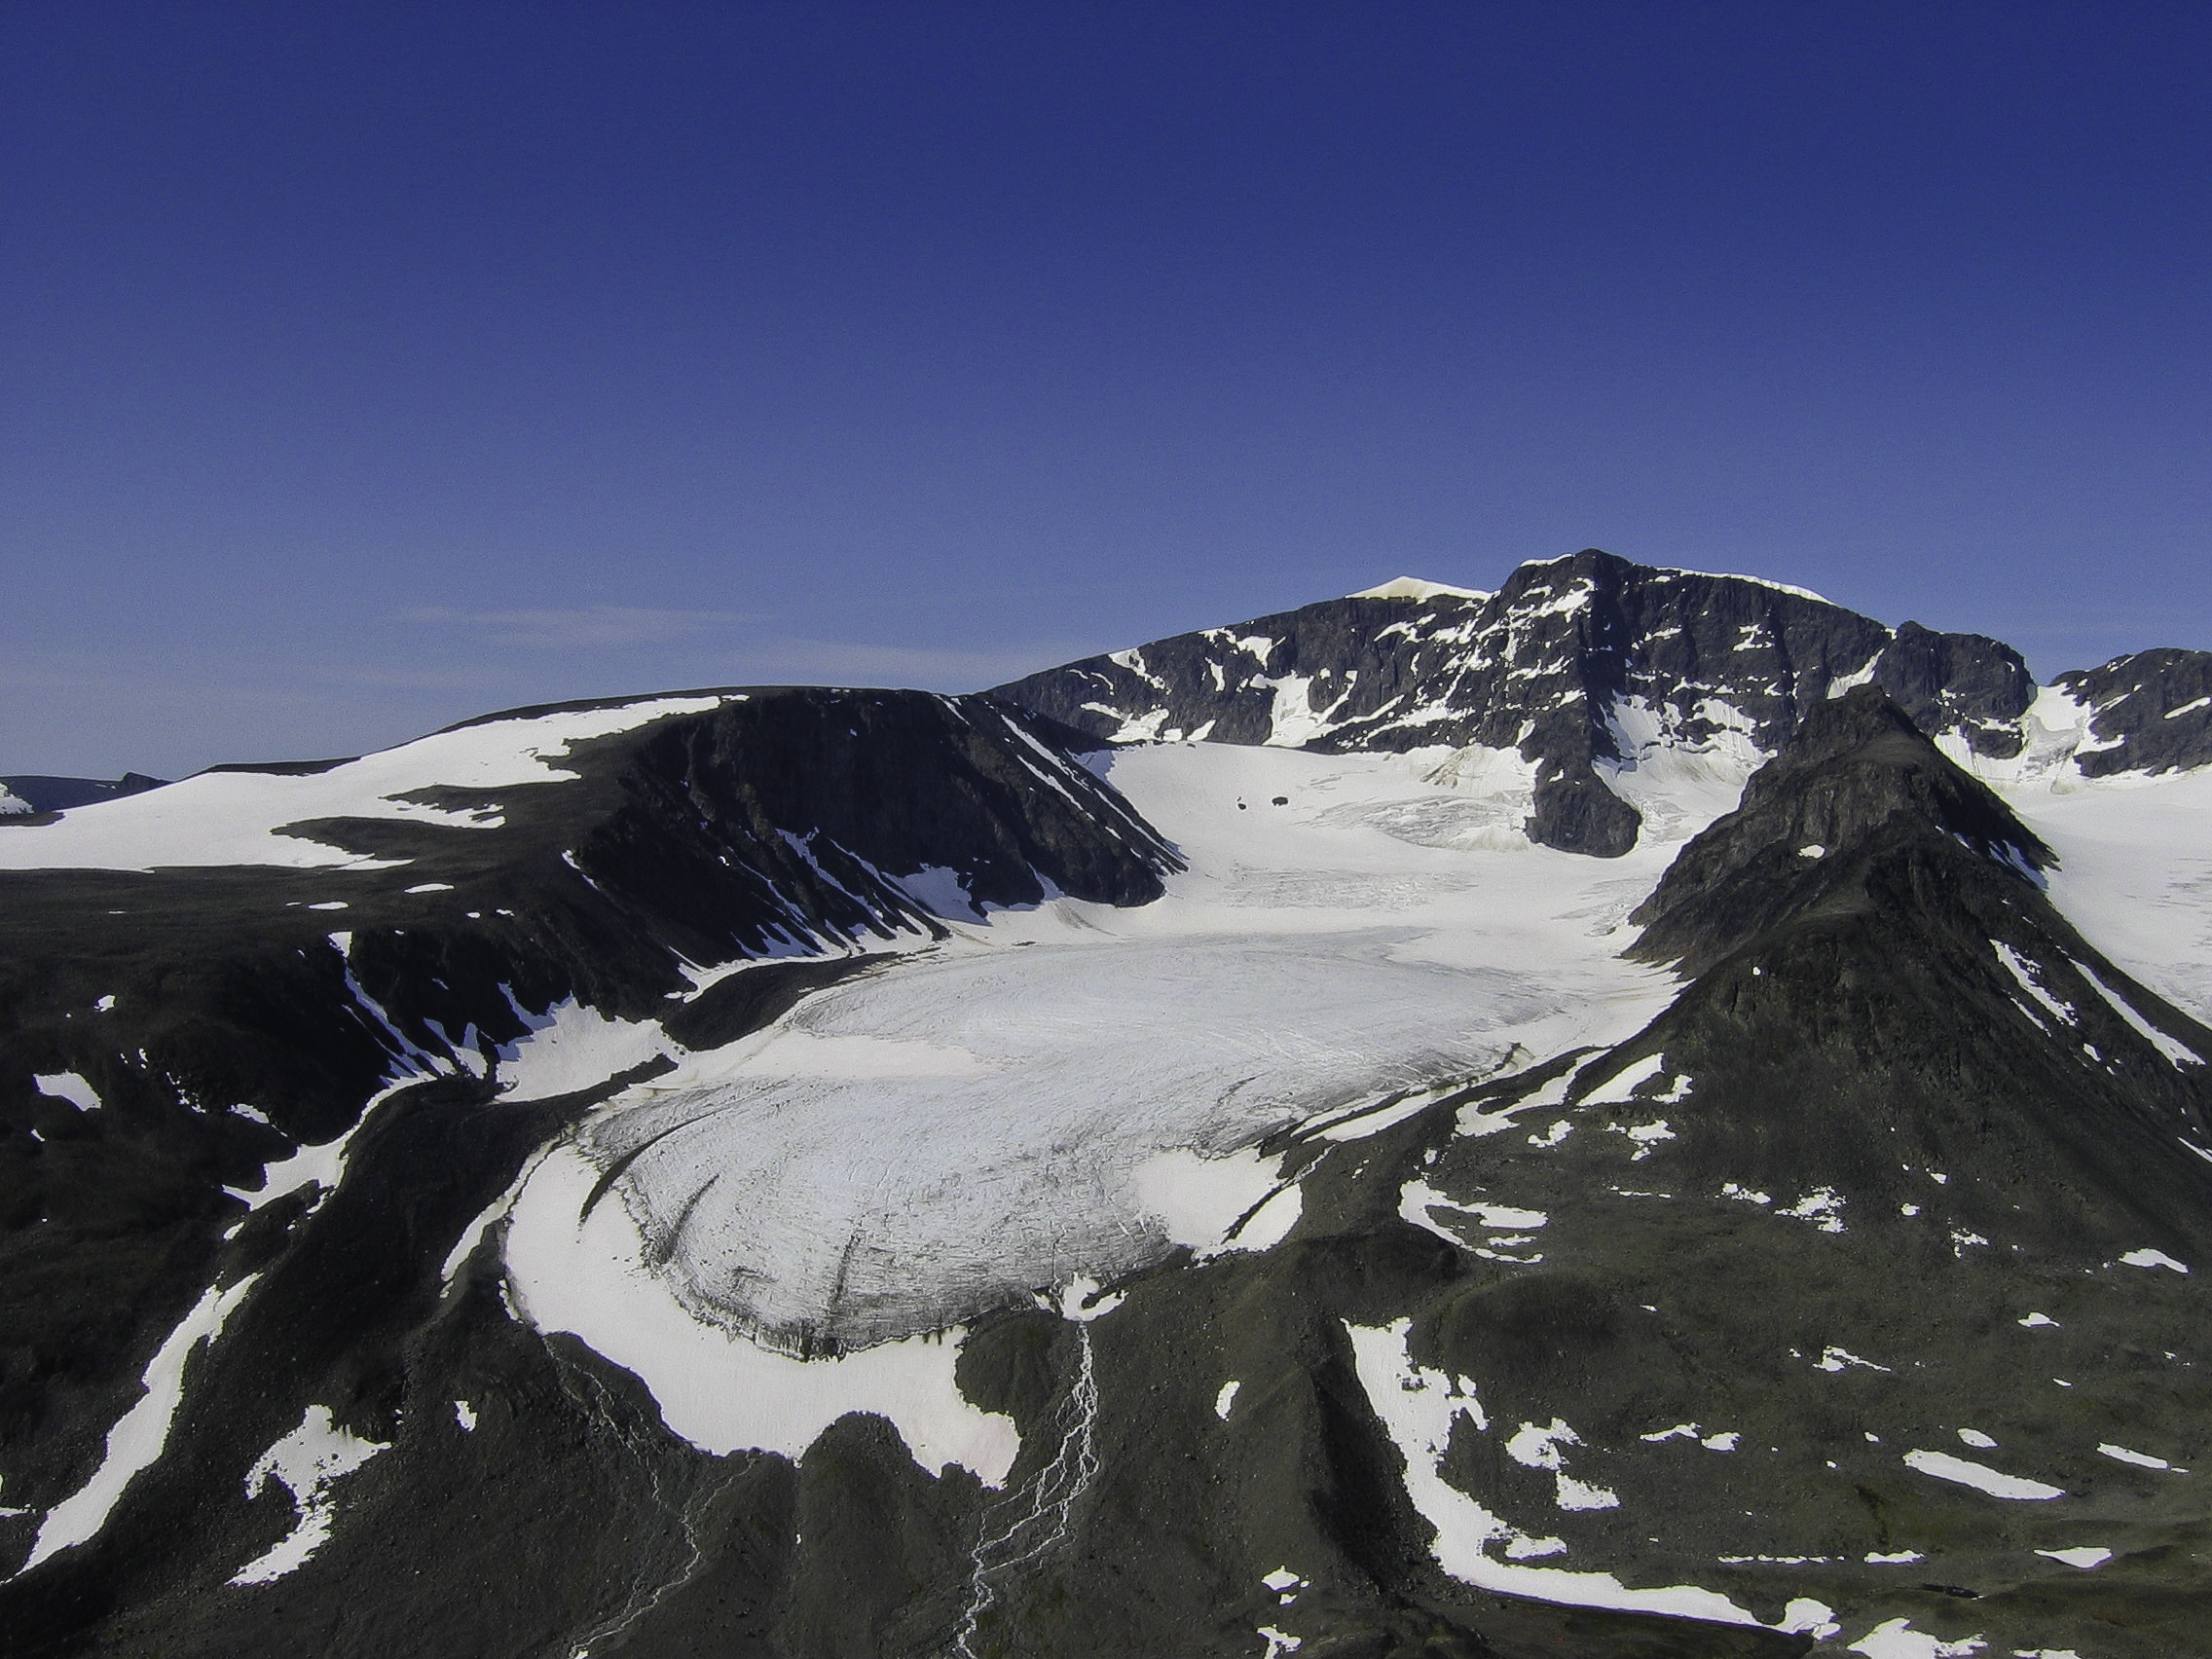
\includegraphics[width=3.in,keepaspectratio=true]{storglaciaren}\qquad
  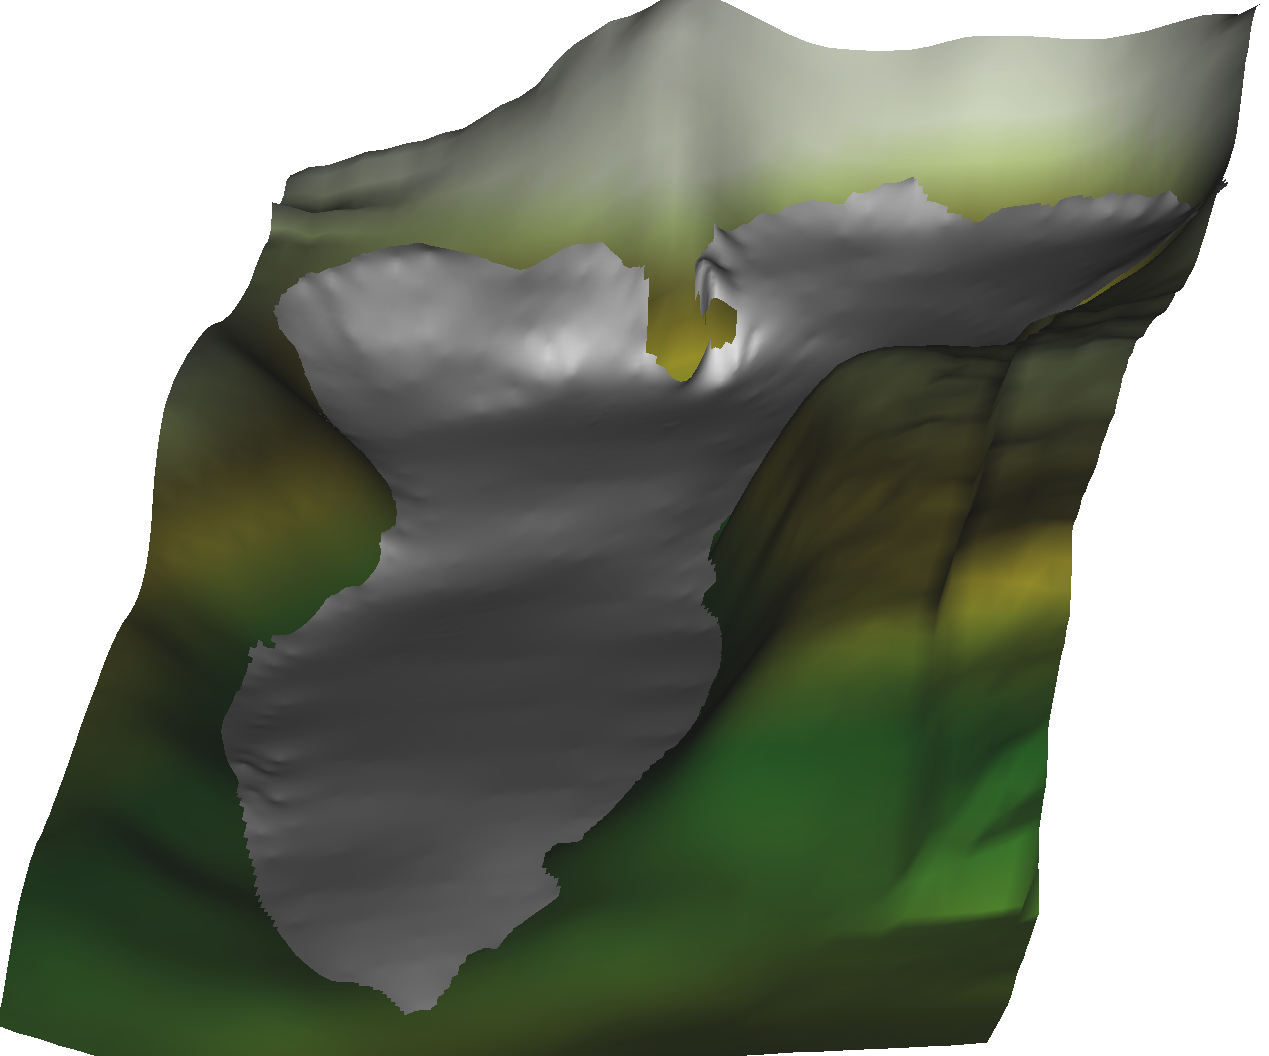
\includegraphics[width=2.75in,keepaspectratio=true]{storglaciaren-dem}
  \caption{Storglaci{\"a}ren, northern Sweden. Left: photo by R. Hock. Right: digital elevation model.}
  \label{fig:storglaciaren}
\end{figure}

The script \texttt{preprocess.sh} in \texttt{examples/storglaciaren} reads the digital elevation model from ASCII files and generates the necessary input files for both the 3-dimensional and the flow-line application. 
